\documentclass{elbioimp2}
\usepackage[utf8]{inputenc}

\usepackage[backend=biber,style=vancouver]{biblatex}
\usepackage{csquotes}
 \usepackage{qcircuit}

\title{The state of Quantum Computing in 2025}
% \shorttitle{Short version of title}
\author{Adam Prior.\affiliation{UrbanFox, Dublin, Ireland}} 
\shortauthor{A. Prior.}
% \elbioimpreceived{19 Sept 2025}  
% \elbioimppublished{19 Sept 2025}
% \elbioimpfirstpage{1}
% \elbioimpvolume{x}
% \elbioimpyear{20xx}
 
\addbibresource{bibliography.bib}

\begin{document}
\setcounter{secnumdepth}{2}


\maketitle

\begin{abstract}
  This paper provides an accessible overview of the current state of quantum computing technologies
  as of September 2025. Aimed at readers with a technical background but no prior experience in quantum
  computing, it reviews foundational concepts, historical advancements, and leading hardware and software platforms. The paper
  also discusses practical challenges, potential applications, and the outlook for future developments in the field.

  \keywords{Quantum Computing; Quibits; Decoherence; robotics}
\end{abstract}

\section{. Introduction}
Define Quantum Advantage here.
Define Some other terms here.

todo: add to historical section that Shor's algorithm is somewhat of a benchmark for quantum computing


\section{. Historical Advancements in Quantum Computing}
The first mentions of quantum computation can be traced as far back as the early as 1980s.
In 1980, mathematician Yuri Manin discussed the concept of a quantum computer in his paper
`Computable and Uncomputable'\cite{Manin1980}. Richard Feynman, in 1982, published a paper
`Simulating physics with computers' introducing the idea of simulating
quantum systems using quantum computers\cite{Feynman1982}, highlighting the limitations
of classical computers at simulating the exponentially growing state space of quantum
systems and how quantum systems can be more efficiently simulated. 

Given these initial few years of defining work, the field began
to gain traction, followed by another \textit{10 years} of foundational theoretical developments.
In 1985, David Deutsch further developed the quantum computing theory by rigorously defining the  
Universal Quantum Turing Machine (the quantum analog of a classical Turing machine) capable of
performing any computation that a classical computer can, but more efficiently for certain problems\cite{Deutsch1985}. 
Further theoretical advancements continued with contributions from, reversible quantum computation by Paul Benioff between
1985-1987\cite{BBenioff1987}, the first proposal of a physically realizable quantum computer 
using atoms and photons in 1998\cite{Yamamoto1998}, and attempts to define quantum complexity 
classes in 1989\cite{Bernstein1993} which would eventually lead to the definition of 
Bounded-Error Quantum Polynomial Time (BQP) problems, an important class of problems in complexity
theory that can be efficiently solved by quantum computers in polynomial time.

It was not until 1992 that the first quantum algorithm was proposed by Deutsch and Jozsa\cite{Deutsch1992},
demonstrating that quantum computers could solve certain problems more efficiently than classical computers 
(quantum advantage). While this algorithm has very limited practical applications, it paved the way for more 
impactful algorithms.
The most famous of these is Shor's algorithm, proposed by Peter Shor in 1994\cite{Shor1994}. Shor's algorithm 
is an efficient quantum algorithm for integer factorization in polynomial time, versus the best-known classical
algorithms which run in sub-exponential time. This algoirithm in some sense `proved' the potential of quantum computing
to solve practical problems that are intractable for classical computers, particularly in the context of cryptography, as
many encryption schemes rely on the difficulty of factoring large integers. 
Another significant algorithm is Grover's algorithm, proposed by Lov Grover two years later\cite{Grover1996}, which provides
a quadratic speedup for unstructured search problems.


\section{. Fundamentals of Quantum Computing}
This document is a template for \LaTeX. 
Please use the electronic version of this document as a
template when you produce your manuscript for submission to the
\emph{Nordic Machine Intelligence}. The paper size is A4 (21 × 
29.7~cm).

The introduction section of your paper should include the necessary
background information, including an adequate review of earlier
findings and the justification for conducting this study.

\subsection{. Qubits and their construction}
All figures should be numbered consecutively with the figure legend
indented 0.5\,cm on each side. See figure commented fig for an example.
Figures may be in color or black and white and must be of such quality
that they produce clear and sharp printouts on an ordinary (color)
laser printer.


\section{. Leading Quantum Hardware Platforms}
Use this section to present the results from the measurements or
studies that were described in the last section, but without going
into any discussion about the results.

% \begin{figure}[htp]
%   \centering
%   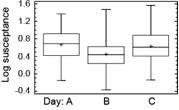
\includegraphics[width=0.7\columnwidth]{assets/test-ill}
%   \caption{Box-plot showing median value (line), mean value (cross),
%     middle 50\,\% (box) and smallest and largest point within 
%     1.5~interquartiles from the box (whiskers) of all measurements
%     on days A, B and~C.\label{box-plot}}
% \end{figure}


\begin{figure}[h]
  \centering
    \scalebox{1.5}{
      \Qcircuit @C=2em @R=1em {
        & \ctrl{2} & \targ & \gate{U} & \qw \\
        & \qw & \ctrl{-1} & \qw & \qw \\
        & \targ & \ctrl{-1} & \ctrl{-2} & \qw \\
        & \qw & \ctrl{-1} & \qw & \qw
      }
  }
  \caption{Example of a simple quantum circuit. Each horizontal line represents a qubit, and the symbols show basic operations that can be performed on them.}
\end{figure}

\section{. Practical Challenges in Quantum Computing}
To achieve a genuine exponential speedup with a quantum algorithm, it is not enough to just put data into superposition — 
the critical ingredient is finding a global structure in the problem that quantum interference can exploit efficiently. In practice, this means (i) encoding the 
problem into a quantum state space so that relevant solutions are distributed across amplitudes, (ii) having an operation that introduces a regular, 
exploitable pattern (periodicity, symmetry, or spectral property), and (iii) applying transformations — such as the Quantum Fourier Transform, amplitude amplification, 
or quantum walks — that sharpen interference in favor of the correct answers while suppressing others. Exponential gains only arise when the quantum evolution can 
collapse an exponentially large superposition into a sharply distinguishable measurement outcome in polynomial time, something that classical algorithms cannot 
replicate without exponential resources. In short, exponential quantum advantage emerges when there is a hidden algebraic or structural feature in the problem that 
quantum linear algebra can amplify, rather than from brute-force parallelism alone.



\section{Potential Applications of Quantum Computing}
The journal of \emph{Nordic Machine Intelligence} uses primarily the Vancouver
style of references with numbers in square brackets in the text and a
numbered list in the Reference section.\cite{biomed-req} However, using the
Harvard reference style will also be accepted in some cases.

\section{Future Outlook and Developments}


\newpage
\nocite{*}
\printbibliography
\end{document}
